\documentclass[12pt, twoside]{article}
\usepackage[letterpaper, margin=1in, headsep=0.2in]{geometry}
\setlength{\headheight}{0.6in}
%\usepackage[english]{babel}
\usepackage[utf8]{inputenc}
\usepackage{microtype}
\usepackage{amsmath}
\usepackage{amssymb}
%\usepackage{amsfonts}
\usepackage{siunitx} %units in math. eg 20\milli\meter
\usepackage{yhmath} % for arcs, overparenth command
\usepackage{tikz} %graphics
\usetikzlibrary{quotes, angles}
\usepackage{graphicx} %consider setting \graphicspath{{images/}}
\usepackage{parskip} %no paragraph indent
\usepackage{enumitem}
\usepackage{multicol}
\usepackage{venndiagram}

\usepackage{fancyhdr}
\pagestyle{fancy}
\fancyhf{}
\renewcommand{\headrulewidth}{0pt} % disable the underline of the header
\raggedbottom
\hfuzz=2mm %suppresses overfull box warnings

\usepackage{hyperref}

\fancyhead[LE]{\thepage}
\fancyhead[RO]{\thepage \\ Name: \hspace{4cm} \,\\}
\fancyhead[LO]{BECA / Dr. Huson / Geometry\\*  Unit 6: Analytic geometry\\* 13 January 2023}

\begin{document}

\subsubsection*{6.13 Test: Analytic geometry \hfill 8.F.A.3}
\begin{enumerate}

\item A line is plotted in the graph below.
\begin{multicols}{2}
    \begin{enumerate}[itemsep=0.5cm]
      \item Write down the $y$-intercept of the line.
      \item What is the slope of the line?
      \item What is the $x$-intercept of the line?
      \item Write down its equation in slope-intercept form.
      \end{enumerate}
    \begin{flushright}
    \begin{tikzpicture}[scale=0.8]
      \draw [help lines] (-1,-4) grid (6,3);
      \draw [thick, ->] (-1.2,0) -- (6.4,0) node [below right] {$x$};
      \draw [thick, ->] (0,-4.2)--(0,3.4) node [right] {$y$};
      \draw [fill] (0,-3) circle [radius=0.05] node[below right] {$(0,-3)$};
      \draw [fill] (2,0) circle [radius=0.05] node[below right] {$(2,0)$};
      \draw [<->, thick, domain=-0.5:4.3] plot (\x,1.5*\x-3);
    \end{tikzpicture}
    \end{flushright}
  \end{multicols} \vspace{2cm}

\item Find the slope of the line through the points $(-2, 3)$ and $(4, 5)$. \vspace{3cm}

\item A line has a slope of $\displaystyle \frac{3}{5}$ and passes through the point $(10, 2)$. 
  \begin{enumerate}[itemsep=1cm]
      \item Write the equation of the line in the form $(y-y_0)=m(x-x_0)$.
      \item Rewrite the equation in the form $y=mx+b$. \vspace{4cm}
  \end{enumerate}

\newpage
\subsubsection*{The midpoint formula \hfill HSG.GPE.B.6}
\item In the diagram below, $\overline{AB}$ has endpoints with coordinates $A(-3,1)$ and $B(5,7)$. Find the coordinates of the midpoint $M$ of $\overline{AB}$. Mark and label it on the graph.
\begin{flushright}
  \begin{tikzpicture}[scale=.6]
    \draw [help lines] (-4,-1) grid (7,8);
    \draw [thick, <->] (-4.4,0) -- (7.4,0) node [below right] {$x$};
    \draw [thick, <->] (0,-1.4)--(0,8.4) node [left] {$y$};
    \draw [thick] (-3,1)--(5,7);
    \draw [fill] (-3,1) circle [radius=0.1] node[above left] {$A$};
    \draw [fill] (5,7) circle [radius=0.1] node[below right] {$B$};
  \end{tikzpicture}
\end{flushright}

\item Find the midpoint of $\overline{PQ}$ if $P(5,11)$ and $Q(1,4)$. \vspace{4cm}

\item Given the midpoint $M(6,4)$ of $\overline{AB}$ with $A(2,3)$. Find the coordinates of point $B$. The use of the grid below is optional.
  \begin{flushright}
    \begin{tikzpicture}[scale=.635]
    \draw [help lines] (0,0) grid (11,11);
    \draw [thick, ->] (0,0) -- (11.4,0) node [below right] {$x$};
    \draw [thick, ->] (0,0)--(0,11.4) node [right] {$y$};
    \foreach \x in {1,...,11}
    \draw[shift={(\x,0)}] (0pt,-3pt)--(0pt,3pt) node[below=5pt] {$\x$};
    \foreach \y in {1,...,11}
    \draw[shift={(0,\y)}] (-3pt,0pt)--(3pt,0pt) node[left=5pt] {$\y$};
    \end{tikzpicture}
  \end{flushright}

\newpage
\subsubsection*{The distance formula \hfill 8.G.B.8}
\item Use the distance formula to find the length of $\overline{RS}$ if $R(1,17)$ and $S(9,2)$. \vspace{5cm}

\item Graph and label $\triangle ABC$, $A(2,2)$, $B(2,10)$, $C(8,2)$.
\begin{multicols}{2}
  \begin{flushleft}
    \begin{tikzpicture}[scale=.6]
    \draw [help lines] (0,0) grid (10,10);
    \draw [thick, ->] (0,0) -- (10.4,0) node [below right] {$x$};
    \draw [thick, ->] (0,0)--(0,10.4) node [right] {$y$};
    \foreach \x in {1,...,10}
    \draw[shift={(\x,0)}] (0pt,-3pt)--(0pt,3pt) node[below=5pt] {$\x$};
    \foreach \y in {1,...,10}
    \draw[shift={(0,\y)}] (-3pt,0pt)--(3pt,0pt) node[left=5pt] {$\y$};
    \end{tikzpicture}
  \end{flushleft}
    Find the lengths of its sides.
    \begin{enumerate}[itemsep=0.5cm]
      \item $AB=$
      \item $AC=$
      \item $BC=$
    \end{enumerate}
  \end{multicols}

\subsubsection*{Parallel and perpendicular slopes \hfill HSG.GPE.B.5}
\item The slope of a line is $m= -\frac{3}{5}$. What is the slope of the line parallel to it? \vspace{2cm}
\item What is the slope a line perpendicular to the line $y=2x+7$?

\newpage
\subsubsection*{Systems of equations \hfill HSG.REI.C.6}
\item Lenny buys fruit for a picnic. Oranges cost \$1 and pineapples cost \$2 each. The total cost is \$10 for seven pieces of fruit. Find the number of each kind of fruit purchased.
  \begin{flushright}
    \begin{tikzpicture}[scale=.65]
      \draw [help lines] (0,0) grid (12,12);
      \draw [thick, ->] (0,0) -- (12.4,0) node [above right] {$x$};
      \draw [thick, ->] (0,0)--(0,12.4) node [right] {$y$};
      \foreach \x in {1,...,12}
      \draw[shift={(\x,0)}] (0pt,-3pt)--(0pt,3pt) node[below=5pt] {$\x$};
      \foreach \y in {1,...,12}
      \draw[shift={(0,\y)}] (-3pt,0pt)--(3pt,0pt) node[left=5pt] {$\y$};
    \end{tikzpicture}
  \end{flushright}

\item Graph and label the two equations. Mark their intersection as an ordered pair.
  \begin{multicols}{2}
    $f(x) = x-3$ \\
    $g(x) = -\frac{3}{5}x+5$
  \end{multicols}
  \begin{center}
  \begin{tikzpicture}[scale=.635]
    \draw [help lines] (-8,-6) grid (10,8);
    \draw [thick, ->] (-8.2,0) -- (10.4,0) node [below right] {$x$};
    \draw [thick, ->] (0,-6.2)--(0,8.4) node [left] {$y$};
  \end{tikzpicture}
  \end{center}

\end{enumerate}
\end{document}